\documentclass[dcc]{fcfmcourse}
\usepackage{teoria}
\usepackage[utf8x]{inputenc}
\usepackage{amsmath}
\usepackage{amsfonts,setspace}
\usepackage{listings}
\usepackage{color}
\usepackage{epstopdf}

\definecolor{pblue}{rgb}{0.13,0.13,1}
\definecolor{pgreen}{rgb}{0,0.5,0}
\definecolor{porange}{rgb}{0.9,0.5,0}
\definecolor{pgrey}{rgb}{0.46,0.45,0.48}

\lstset{language=Java,
  showspaces=false,
  showtabs=false,
  breaklines=true,
  showstringspaces=false,
  breakatwhitespace=true,
  commentstyle=\color{porange},
  keywordstyle=\color{pblue},
  stringstyle=\color{pgreen},
  basicstyle=\ttfamily,
  moredelim=[il][\textcolor{pgrey}]{$ $},
  moredelim=[is][\textcolor{pgrey}]{\%\%}{\%\%}
}

\newenvironment{codebox} {\small \ttfamily \obeylines \begingroup \setstretch{-2.4}} {\endgroup}

\title{Preparación Control 2}
\course[CC3001]{Algoritmos y Estructuras de Datos}
\professor{Nelson Baloian}
\professor{Patricio Poblete}
\assistant{Manuel Cáceres}
\assistant{Sebastián Ferrada}
\assistant{Sergio Peñafiel}

% Si pasas el comando usedate a la clase, la fecha aparecerá bajo la lista de auxiliares.
% Puedes usar el formato de fecha por defecto de latex (y traducirla usando babel)
% o puedes escribir lo que quieras con el comando \date.
% \date{1 de Septiembre, 2015}


\begin{document}
\maketitle

\vspace{-1ex}
\begin{problems}
\problem Problema 1

Para el siguiente grafo:

\begin{center}
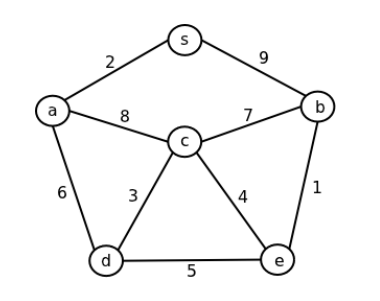
\includegraphics[scale=.7]{imagenes/grafo.PNG}
\end{center}

considere que los valores en los arcos son pesos o costos, y muestre paso a paso la construcción del árbol cobertor mínimo usando los algoritmos de Kruskal y Prim

\problem Problema 2

Implemente el método \texttt{public void eliminar(int i)} del TDA Cola de Prioridad, implementada con un heap (suponga que el arreglo que contiene a la cola se llama \texttt{heap}). Este método debe eliminar el i-ésimo elemento del heap y luego retornar la condición de heap a la cola.

Su algoritmo debe tomar a lo más tiempo $\mathcal{O}(\log n)$, donde $n$ de elementos en la cola de prioridad al momento de realizar la eliminación. Muestre que su implementación cumple con la cota temporal exigida.

\problem Problema 3

Implemente el método \texttt{Nodo podarMayores(Nodo raiz, int valor)}
El método debe eliminar de un árbol de búsqueda binaria (ABB), referenciado por raíz, todos aquellos nodos cuyo identificador sea mayor que valor. El árbol resultante también tiene que ser un ABB. Note que \textbf{NO} necesariamente hay un nodo en el ABB original cuyo identificador sea valor.

Su algoritmo debe tomar tiempo proporcional a la altura del árbol original, por lo tanto no sirve leer uno a uno los nodos del árbol y quedarse con los menores que valor. Muestre que su implementación cumple con la cota temporal exigida

\problem Problema 4 

Se tiene un conjunto de $n$ tornillos y otro de $n$ tuercas en los cuales cada tornillo se puede atornillar en exactamente una tuerca.\\
Este problema consiste en encontrar los pares correspondientes de tornillos y tuercas. Para realizar esto es posible determinar si a cierto tornillo le queda grande una tuerca, le queda chica, o es su tuerca correspondiente. Sin embargo, no es posible comparar tamaños entre dos tuercas o entre dos tornillos.\\

Implemente un algoritmo que funcione en tiempo $\mathcal{O}(n\log n)$.\\
Hint: Ordene

\end{problems}

\end{document}

